\documentclass[a4paper,12pt]{article}[abntex2]
\bibliographystyle{abntex2-alf}
\usepackage{siunitx} % Fornece suporte para a tipografia de unidades do Sistema Internacional e formatação de números
\usepackage{booktabs} % Melhora a qualidade das tabelas
\usepackage{tabularx} % Permite tabelas com larguras de colunas ajustáveis
\usepackage{graphicx} % Suporte para inclusão de imagens
\usepackage{newtxtext} % Substitui a fonte padrão pela Times Roman
\usepackage{ragged2e} % Justificação de texto melhorada
\usepackage{setspace} % Controle do espaçamento entre linhas
\usepackage[a4paper, left=3.0cm, top=3.0cm, bottom=2.0cm, right=2.0cm]{geometry} % Personalização das margens do documento
\usepackage{lipsum} % Geração de texto dummy 'Lorem Ipsum'
\usepackage{fancyhdr} % Customização de cabeçalhos e rodapés
\usepackage{titlesec} % Personalização dos títulos de seções
\usepackage[portuguese]{babel} % Adaptação para o português (nomes e hifenização
\usepackage{hyperref} % Suporte a hiperlinks
\usepackage{indentfirst} % Indentação do primeiro parágrafo das seções
\sisetup{
  output-decimal-marker = {,},
  inter-unit-product = \ensuremath{{}\cdot{}},
  per-mode = symbol
}
\DeclareSIUnit{\real}{R\$}
\newcommand{\real}[1]{R\$#1}
\usepackage{float} % Melhor controle sobre o posicionamento de figuras e tabelas
\usepackage{footnotehyper} % Notas de rodapé clicáveis em combinação com hyperref
\hypersetup{
    colorlinks=true,
    linkcolor=black,
    filecolor=magenta,      
    urlcolor=cyan,
    citecolor=black,        
    pdfborder={0 0 0},
}
\usepackage[normalem]{ulem} % Permite o uso de diferentes tipos de sublinhados sem alterar o \emph{}
\makeatletter
\def\@pdfborder{0 0 0} % Remove a borda dos links
\def\@pdfborderstyle{/S/U/W 1} % Estilo da borda dos links
\makeatother
\onehalfspacing
\setlength{\headheight}{14.49998pt}

\begin{document}

\begin{titlepage}
    \centering
    \vspace*{1cm}
    \Large\textbf{INSPER – INSTITUTO DE ENSINO E PESQUISA}\\
    \Large \textbf{ECONOMIA}\\
    \vspace{1.5cm}
    \Large\textbf{Tradução  de Mastering Metrics ; The Path from Cause to Effect (Joshua D. Angrist)}\\
    \textbf{PIBIC}\\
    \vspace{1.5cm}
    Prof. Dr Paulo Cilas Marques Filho\\
    \vfill
    \normalsize
    Hicham Munir Tayfour, \href{mailto:hichamt@al.insper.edu.br}{hichamt@al.insper.edu.br}\\
    5º Período - Economia \\
    \vfill
    Goiânia\\
    Junho/2024
\end{titlepage}

\newpage
\tableofcontents
\thispagestyle{empty} % This command removes the page number from the table of contents page
\newpage
\setcounter{page}{1} % This command sets the page number to start from this page
\justify
\onehalfspacing

\pagestyle{fancy}
\fancyhf{}
\rhead{\thepage}

\section{Introdução}

\textbf{MESTRE PO CEGO:} Feche os olhos. O que você ouve?

\textbf{JOVEM KWAI CHANG CAINE:} Eu ouço a água, eu ouço os pássaros.

\textbf{MESTRE PO:} Você ouve o seu próprio coração bater?

\textbf{KWAI CHANG CAINE:} Não.

\textbf{MESTRE PO:} Você ouve o gafanhoto que está aos seus pés?

\textbf{KWAI CHANG CAINE:} Velho, como é que você ouve essas coisas?

\textbf{MESTRE PO:} Jovem, como é que você não as ouve?

\emph{Kung Fu, Piloto}

A reputação dos economistas por pessimismo é injusta. A economia é tão empolgante quanto qualquer ciência pode ser: o mundo é nosso laboratório, e as diversas pessoas nele são nossos sujeitos.

A emoção em nosso trabalho vem da oportunidade de aprender sobre causa e efeito nos assuntos humanos. As grandes questões do momento são nossas questões: Uma política monetária frouxa vai estimular o crescimento econômico ou apenas alimentar a inflação? Os agricultores de Iowa e o presidente do Federal Reserve querem saber. O seguro de saúde obrigatório realmente fará os americanos mais saudáveis? Essas discussões políticas alimentam os debates nos programas de rádio. No entanto, abordamos essas questões com calma, armados não com paixão, mas com dados.

O uso de dados pelos economistas para responder perguntas de causa e efeito constitui o campo da econometria aplicada, conhecido por estudantes e mestres como \emph{'metrics'}. As ferramentas do comércio de \emph{'metrics'} são análises de dados disciplinadas, combinadas com o maquinário da inferência estatística. Há também um aspecto místico em nosso trabalho: estamos atrás da verdade, mas a verdade não é revelada por completo, e as mensagens que os dados transmitem requerem interpretação. Nesse espírito, nos inspiramos na jornada de Kwai Chang Caine, herói da clássica série de TV \emph{Kung Fu}. Caine, um monge Shaolin de raça mista, vaga em busca de seu meio-irmão nascido nos EUA no oeste americano do século XIX. Enquanto ele busca, Caine questiona tudo o que vê nos assuntos humanos, descobrindo relacionamentos ocultos e significados mais profundos. Assim como a jornada de Caine, o Caminho de \emph{'Metrics'} é iluminado por perguntas.

\textbf{Other Things Equal}

Em um desenvolvimento perturbador de que você pode ter ouvido falar, a proporção de estudantes universitários americanos que concluem seus cursos de forma oportuna deu uma guinada acentuada para baixo. Políticos e analistas de políticas culpam a queda nas taxas de graduação universitária por uma combinação perniciosa de aumentos nas mensalidades e os grandes empréstimos estudantis que muitos alunos usam para financiar seus estudos. Talvez o aumento dos empréstimos estudantis desvie alguns que, de outra forma, permaneceriam no caminho certo. O fato de que os alunos mais propensos a abandonar a escola frequentemente carregam grandes empréstimos estudantis parece substanciar essa hipótese.

Você preferiria pagar a faculdade com riquezas herdadas do que com dinheiro emprestado, se puder. Como discutiremos em detalhes, no entanto, a educação provavelmente aumenta os ganhos o suficiente para tornar o pagamento do empréstimo suportável para a maioria dos graduados. Como então devemos interpretar a correlação negativa entre o fardo da dívida e as taxas de graduação universitária? A dívida causa abandono escolar? A primeira pergunta a fazer neste contexto é quem empresta mais. Estudantes que emprestam muito geralmente vêm de famílias de renda média e baixa, uma vez que famílias mais ricas têm mais poupança. Por muitos motivos, os alunos de famílias de baixa renda são menos propensos a concluir um curso do que aqueles de famílias de alta renda, independentemente de terem emprestado muito. Portanto, devemos ser céticos em relação às alegações de que altos encargos de dívida causam taxas mais baixas de conclusão universitária quando essas alegações são baseadas apenas em comparações de taxas de conclusão entre aqueles com mais ou menos dívida. Em virtude da correlação entre a origem familiar e a dívida universitária, o contraste nas taxas de graduação entre aqueles com e sem empréstimos estudantis não é uma comparação de "outras coisas iguais".

Como estudantes universitários se especializando em economia, aprendemos pela primeira vez a ideia de "outras coisas iguais" pelo seu nome em latim, \emph{ceteris paribus}. Comparações feitas sob condições de \emph{ceteris paribus} têm uma interpretação causal. Imagine dois alunos idênticos em todos os aspectos, cujas famílias têm os mesmos recursos financeiros e cujos pais têm níveis de educação semelhantes. Um desses gêmeos virtuais financia a faculdade emprestando e o outro com poupança. Porque eles são iguais em todos os outros aspectos (a avó deu a ambos um pequeno ninho de poupança), as diferenças em seu desempenho educacional podem ser atribuídas ao fato de que apenas um deles tomou empréstimo. Até hoje, nos perguntamos por que tantos estudantes de economia encontram essa ideia central primeiro em latim; talvez seja uma conspiração para mantê-los de pensar sobre isso. Porque, como essa comparação hipotética sugere, comparações reais de "outras coisas iguais" são difíceis de realizar, alguns diriam até \emph{impossibile} (isso é italiano, não latim, mas pelo menos ainda é falado).

Difícil de realizar, talvez, mas não necessariamente impossível. A arte de \emph{'metrics'} usa dados para chegar a "outras coisas iguais" apesar dos obstáculos — chamados viés de seleção ou viés de variáveis omitidas — encontrados no caminho que vai de números brutos a conhecimento causal confiável. O caminho para o entendimento causal é áspero e sombrio, contornando os obstáculos do viés de seleção. E ainda assim, mestres de \emph{'metrics'} percorrem esse caminho com confiança e humildade, ligando com sucesso causa e efeito.

Nossa primeira linha de ataque ao problema da causalidade é um experimento randomizado, frequentemente chamado de ensaio randomizado. Em um ensaio randomizado, os pesquisadores mudam as variáveis causais de interesse (digamos, a disponibilidade de ajuda financeira para a faculdade) para um grupo selecionado usando algo como um lançamento de moeda. Ao mudar as circunstâncias aleatoriamente, tornamos altamente provável que a variável de interesse não esteja relacionada a muitos outros fatores que determinam os resultados que queremos estudar. A atribuição aleatória não é o mesmo que manter tudo o mais constante, mas tem o mesmo efeito. A manipulação aleatória faz com que "outras coisas iguais" prevaleçam, em média, nos grupos que experimentaram ou não a manipulação. Como explicamos no Capítulo 1, "em média" geralmente é bom o suficiente.

\begin{figure}[H]
    \centering
    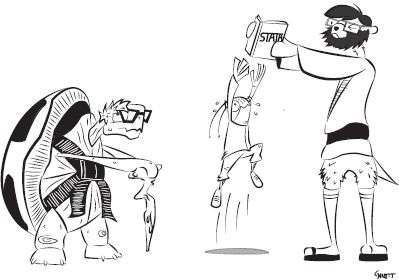
\includegraphics[width=0.75\textwidth]{PIBIC/Tradução Mater Metrics/image.png}
    
    \end{figure}

Os ensaios randomizados têm lugar de destaque em nosso kit de ferramentas de \emph{'metrics'}. Infelizmente, os experimentos sociais randomizados são caros de realizar e podem demorar para dar frutos, enquanto os fundos de pesquisa são escassos e a vida é curta. Muitas vezes, portanto, os mestres de \emph{'metrics'} recorrem a desenhos de pesquisa menos poderosos, mas mais acessíveis. Mesmo quando não podemos randomizar de forma prática, no entanto, ainda sonhamos com os ensaios que gostaríamos de fazer. A noção de um experimento ideal disciplina nossa abordagem à pesquisa econométrica. \emph{Mastering 'Metrics} mostra como a aplicação sábia de nossas cinco ferramentas econométricas favoritas nos aproxima o máximo possível do poder revelador de causalidade de um experimento real.

Nossas ferramentas econométricas favoritas são ilustradas aqui através de uma série de estudos econométricos bem elaborados e importantes. Avaliadas pelo Grande Mestre Oogway do Palácio de Jade do \emph{Kung Fu Panda}, essas investigações dos efeitos causais são distinguidas por sua excelência. Os métodos que eles usam — atribuição aleatória, regressão, variáveis instrumentais, desenhos de descontinuidade de regressão e diferenças-em-diferenças — são os \emph{Furious Five} da pesquisa econométrica. Para começar, motivado pelo debate contemporâneo americano sobre saúde, o primeiro capítulo descreve dois experimentos sociais que revelam se, como muitos formuladores de políticas acreditam, o seguro de saúde realmente ajuda aqueles que o possuem a permanecerem saudáveis. Os capítulos 2–5 colocam nossas outras ferramentas em prática, elaborando respostas para perguntas importantes, que vão desde os benefícios de frequentar faculdades particulares e escolas secundárias seletivas até os custos do consumo de álcool por adolescentes e os efeitos das injeções de liquidez pelo banco central.

Nosso capítulo final coloca os \emph{Furious Five} à prova ao retornar ao campo da educação. Em média, graduados universitários ganham cerca de duas vezes mais do que graduados do ensino médio, uma diferença de ganhos que só parece estar aumentando. O Capítulo 6 pergunta se essa diferença é evidência de um grande retorno causal para a educação ou meramente uma reflexão das muitas outras vantagens que aqueles com mais educação podem ter (como pais mais educados). A relação entre escolaridade e ganhos pode ser avaliada em uma base de \emph{ceteris paribus}, ou os obstáculos do viés de seleção bloquearão para sempre nosso caminho? O desafio de quantificar a ligação causal entre escolaridade e ganhos fornece um teste cativante para as ferramentas de \emph{'metrics'} e os mestres que as utilizam.

\newpage

\section{Ensaios Randomizados}

\textbf{KWAI CHANG CAINE:} O que acontece na vida de um homem já está escrito. Um homem deve seguir pela vida conforme sua vontade.

\textbf{VELHO:} No entanto, cada um é livre para viver como escolher. Embora pareçam opostos, ambos são verdadeiros.

\emph{Kung Fu, Piloto}

\textbf{Nosso Caminho}

Nosso caminho começa com a atribuição aleatória experimental, tanto como uma estrutura para questões causais quanto como um parâmetro pelo qual os resultados de outros métodos são julgados. Ilustramos o poder impressionante da atribuição aleatória através de duas avaliações randomizadas dos efeitos do seguro de saúde. O apêndice deste capítulo também usa a estrutura experimental para revisar os conceitos e métodos de inferência estatística.

\subsection{Na Saúde e na Doença (Seguro de Saúde)}

O Affordable Care Act (ACA) tem se mostrado uma das inovações políticas mais controversas e interessantes que já vimos. O ACA exige que os americanos comprem seguro de saúde, com uma penalidade fiscal para aqueles que não aderirem voluntariamente. A questão do papel adequado do governo no mercado de saúde possui muitos ângulos. Um deles é o efeito causal do seguro de saúde na saúde. Os Estados Unidos gastam uma parte maior do seu PIB em cuidados de saúde do que outras nações desenvolvidas, no entanto, os americanos são surpreendentemente menos saudáveis. Por exemplo, os americanos têm mais probabilidade de serem obesos e morrerem mais cedo do que seus primos canadenses, que gastam apenas cerca de dois terços do que os americanos gastam em cuidados de saúde. Os Estados Unidos também são incomuns entre os países desenvolvidos por não terem um esquema de seguro de saúde universal. Talvez haja uma conexão causal aqui.

Os americanos idosos são cobertos por um programa federal chamado Medicare, enquanto alguns americanos pobres (incluindo a maioria das mães solteiras, seus filhos e muitas outras crianças pobres) são cobertos pelo Medicaid. Muitos dos pobres em idade produtiva, no entanto, têm sido por muito tempo não segurados. Na verdade, muitos americanos sem seguro optaram por não participar de um plano de seguro fornecido pelo empregador. Esses trabalhadores, talvez corretamente, contam com os departamentos de emergência dos hospitais, que não podem recusá-los, para atender às suas necessidades de saúde. Mas o departamento de emergência pode não ser o melhor lugar para tratar, digamos, a gripe, ou para gerenciar condições crônicas como diabetes e hipertensão, que são tão prevalentes entre os americanos pobres. O departamento de emergência não é obrigado a fornecer cuidados de longo prazo. Portanto, faz sentido que o seguro de saúde obrigatório pelo governo possa resultar em um dividendo de saúde. O impulso pelo seguro de saúde universal subsidiado decorre em parte da crença de que ele resulta.

A questão de \emph{ceteris paribus} neste contexto contrasta a saúde de alguém com cobertura de seguro com a saúde da mesma pessoa sem seguro (exceto pelo suporte do departamento de emergência). Esse contraste destaca um dilema empírico fundamental: as pessoas estão ou seguradas ou não. Não podemos vê-las nas duas condições ao mesmo tempo nas mesmas circunstâncias exatas.

Em seu célebre poema, "The Road Not Taken", Robert Frost usou a metáfora de uma encruzilhada para descrever os efeitos causais da escolha pessoal:
\begin{quote}
Duas estradas divergiam em um bosque amarelo, \\
E lamentei não poder viajar por ambas \\
E sendo um só viajante, longo fiquei \\
E olhei para uma até onde pude \\
Onde ela se dobrava no matagal;
\end{quote}
O viajante de Frost conclui:
\begin{quote}
Duas estradas divergiam em um bosque, e eu - \\
Eu peguei a menos percorrida, \\
E isso fez toda a diferença.
\end{quote}

O viajante afirma que sua escolha fez diferença, mas, sendo apenas uma pessoa, ele não pode ter certeza. Uma viagem posterior ou um relatório de outros viajantes também não esclareceria isso para ele. Nosso narrador pode estar mais velho e sábio da próxima vez, enquanto outros viajantes podem ter experiências diferentes na mesma estrada. Assim é com qualquer escolha, incluindo aquelas relacionadas ao seguro de saúde: homens sem seguro com doenças cardíacas estariam livres da doença se tivessem seguro? No romance \emph{Light Years}, o narrador irresoluto de James Salter observa: "Atos destroem suas alternativas, esse é o paradoxo." Não podemos saber o que está no fim da estrada não escolhida.

Não podemos saber, mas evidências podem ser consideradas. Este capítulo o levará através de algumas das evidências relacionadas aos caminhos envolvendo seguro de saúde. O ponto de partida é a Pesquisa Nacional de Entrevistas de Saúde (NHIS), uma pesquisa anual da população dos EUA com informações detalhadas sobre saúde e seguro de saúde. Entre muitas outras coisas, o NHIS pergunta: "Você diria que sua saúde em geral é excelente, muito boa, boa, razoável ou ruim?" Usamos esta pergunta para codificar um índice que atribui 5 para excelente saúde e 1 para saúde ruim em uma amostra de respondentes casados do NHIS de 2009 que podem ou não estar segurados. Este índice é nosso desfecho: uma medida que estamos interessados em estudar. A relação causal de interesse aqui é determinada por uma variável que indica a cobertura por seguro de saúde privado. Chamamos essa variável de tratamento, emprestando da literatura sobre ensaios médicos, embora os tratamentos de nosso interesse não precisem ser tratamentos médicos como medicamentos ou cirurgias. Neste contexto, aqueles com seguro podem ser considerados o grupo de tratamento; aqueles sem seguro compõem o grupo de comparação ou controle. Um bom grupo de controle revela o destino dos tratados em um mundo contrafactual onde eles não são tratados.

A primeira linha da Tabela 1.1 compara o índice médio de saúde de americanos segurados e não segurados, com estatísticas tabuladas separadamente para maridos e esposas. Aqueles com seguro de saúde são de fato mais saudáveis do que aqueles sem, uma diferença de cerca de 0,3 no índice para homens e 0,4 no índice para mulheres. Essas são diferenças grandes quando medidas contra o desvio padrão do índice de saúde, que é cerca de 1. (Os desvios padrões, reportados entre colchetes na Tabela 1.1, medem a variabilidade nos dados. O apêndice do capítulo revisa a fórmula relevante.) Esses grandes hiatos podem ser o dividendo de saúde que estamos procurando.

\textbf{Comparações Infrutíferas e Frutíferas}

Comparações simples, como as do topo da Tabela 1.1, são frequentemente citadas como evidência de efeitos causais. Na maioria das vezes, no entanto, tais comparações são enganosas. Mais uma vez, o problema é "outras coisas iguais", ou a falta delas. Comparações entre pessoas com e sem seguro de saúde não são de maçãs com maçãs; tais contrastes são de maçãs com laranjas, ou pior.

Entre outras diferenças, aqueles com seguro de saúde são mais bem educados, têm renda mais alta e têm mais probabilidade de estarem trabalhando do que os não segurados. Isso pode ser visto no painel B da Tabela 1.1, que relata as características médias dos respondentes do NHIS que têm e não têm seguro de saúde. Muitas das diferenças na tabela são grandes (por exemplo, uma diferença de quase 3 anos de escolaridade); a maioria é estatisticamente precisa o suficiente para descartar a hipótese de que essas discrepâncias são meramente achados ao acaso (veja o apêndice do capítulo para uma revisão sobre significância estatística). Não será surpresa para você saber que a maioria das variáveis tabuladas aqui são altamente correlacionadas tanto com a saúde quanto com o status do seguro de saúde. Pessoas mais educadas, por exemplo, tendem a ser mais saudáveis, além de estarem super-representadas no grupo segurado. Isso pode ser porque pessoas mais educadas se exercitam mais, fumam menos e têm mais probabilidade de usar cintos de segurança. Faz sentido que a diferença na saúde entre os respondentes do NHIS segurados e não segurados reflita pelo menos parcialmente a escolaridade extra dos segurados.


\begin{figure}[H]
    \centering
    \caption{Características de saúde e demográficas de casais segurados e não segurados no NHIS} 
    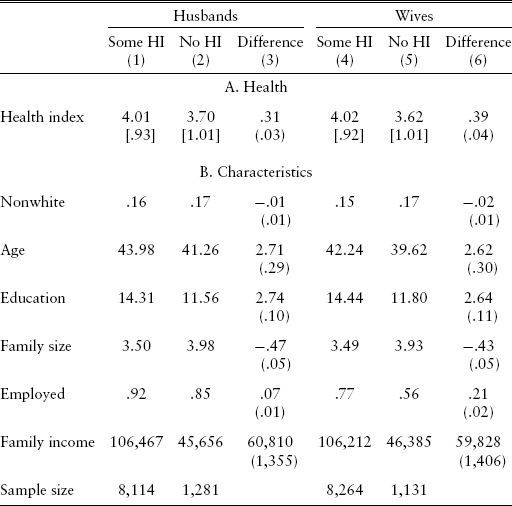
\includegraphics[width=0.75\textwidth]{PIBIC/Tradução Mater Metrics/image2.png}
    
    \footnotesize{Notas: Esta tabela relata as características médias para casais segurados e não segurados na Pesquisa Nacional de Entrevistas de Saúde (NHIS) de 2009. As colunas (1), (2), (4) e (5) mostram as características médias do grupo de indivíduos especificado pelo título da coluna. As colunas (3) e (6) relatam a diferença entre a característica média para indivíduos com e sem seguro de saúde (HI). Desvios padrão estão entre colchetes; erros padrão são reportados entre parênteses.}
    \end{figure}

Nosso esforço para entender a conexão causal entre seguro e saúde é auxiliado por expandir a metáfora das duas estradas de Frost. Usamos a letra Y como abreviação para saúde, a variável de desfecho de interesse. Para deixar claro quando estamos falando de pessoas específicas, usamos subscritos como substitutos para nomes: \( Y_i \) é a saúde do indivíduo \( i \). O desfecho \( Y_i \) é registrado em nossos dados. Mas, ao enfrentar a escolha de pagar ou não pelo seguro de saúde, a pessoa \( i \) tem dois resultados potenciais, dos quais apenas um é observado. Para distinguir um resultado potencial de outro, adicionamos um segundo subscrito: a estrada tomada sem seguro de saúde leva a \( Y_{0i} \) (leia isso como “y-zero-i”) para a pessoa \( i \), enquanto a estrada com seguro de saúde leva a \( Y_{1i} \) (leia isso como “y-um-i”) para a pessoa \( i \). Resultados potenciais estão no fim de cada estrada que se pode tomar. O efeito causal do seguro na saúde é a diferença entre eles, escrito \( Y_{1i} - Y_{0i} \).

Para esclarecer ainda mais, considere a história do estudante do Instituto de Tecnologia de Massachusetts (MIT), Khuzdar Khalat, recentemente chegado do Cazaquistão. O Cazaquistão tem um sistema nacional de seguro de saúde que cobre todos os seus cidadãos automaticamente (embora você não fosse para lá apenas pelo seguro de saúde). Ao chegar em Cambridge, Massachusetts, Khuzdar fica surpreso ao saber que os estudantes do MIT devem decidir se desejam aderir ao plano de seguro de saúde da universidade, pelo qual o MIT cobra uma taxa elevada. Após reflexão, Khuzdar julga que o seguro do MIT vale a pena pagar, já que ele teme infecções respiratórias superiores no frio da Nova Inglaterra. Digamos que \( Y_{0i} = 3 \) e \( Y_{1i} = 4 \) para \( i = \) Khuzdar. Para ele, o efeito causal do seguro é um passo a mais na escala do NHIS:

\begin{equation}
Y_{1,\text{Khuzdar}} - Y_{0,\text{Khuzdar}} = 1.
\end{equation}

A Tabela 1.2 resume essa informação.

\begin{table}[h]
\centering
\caption{Desfechos e tratamentos para Khuzdar e Maria}
\begin{tabular}{lcc}
\hline
 & \textbf{Khuzdar Khalat} & \textbf{Maria Moreño} \\
\hline
Resultado potencial sem seguro: \(Y_{0i}\) & 3 & 5 \\
Resultado potencial com seguro: \(Y_{1i}\) & 4 & 5 \\
Tratamento (status do seguro escolhido): \(D_i\) & 1 & 0 \\
Resultado de saúde atual: \(Y_i\) & 4 & 5 \\
Efeito do tratamento: \(Y_{1i} - Y_{0i}\) & 1 & 0 \\
\hline
\end{tabular}
\end{table}

Vale a pena enfatizar que a Tabela 1.2 é uma tabela imaginária: algumas das informações que ela descreve devem permanecer ocultas. Khuzdar comprará o seguro, revelando seu valor de \(Y_{1i}\), ou não comprará, caso em que seu \(Y_{0i}\) será revelado. Khuzdar percorreu muitas estradas longas e poeirentas no Cazaquistão, mas nem ele pode ter certeza do que está no fim das estradas não tomadas.



\end{document}